\documentclass[useAMS,usenatbib]{mn2e}
\pdfoutput=1
\usepackage[varg]{txfonts}
\usepackage{astrojournals}
\usepackage{graphicx}
\usepackage{microtype}
\usepackage{xcolor}
\usepackage{fixltx2e}
\usepackage{hyperref}
\usepackage{siunitx}
\hypersetup{colorlinks=True, linkcolor=blue!50!black, citecolor=black,
  urlcolor=blue!50!black}

\usepackage[greek,english]{babel} 
\newcommand{\texttheta}{\greektext j\latintext}
\newcommand\thC{\texttheta\textsuperscript{1}\,Ori~C}
\newcommand\elec{\ensuremath{_{\mathrm{e}}}}
\newcommand\Ion[2]{\ensuremath{\mathrm{#1\,\scriptstyle #2}}}
\newcounter{ionstage}
\newcommand{\ion}[2]{% needs to be renewcommand with aastex
  \setcounter{ionstage}{#2}%
  \Ion{#1}{\Roman{ionstage}}}
\newcommand\nii{\ion{N}{2}}
\newcommand\sii{\ion{S}{2}}
\newcommand\oiii{\ion{O}{3}}

\begin{document}

%% Skip over the parts that are already written
\addtocounter{section}{6}
\addtocounter{subsection}{2}
\addtocounter{table}{5}
\addtocounter{figure}{9}


\subsection{A physical model of 177-341}
As an alternative to the purely empirical analysis presented in the previous sections, a different approach to analysing the emission spectrum of the proplyds is through the construction of physical models that combine a priori simulations of radiative transfer, hydrodynamics, and atomic physics in order to predict the density, temperature, and ionization structure of the proplyd flow.  
Such models have previously been applied to the ensemble properties of large numbers of proplyds \citep*{1998ApJ...499..758J, 1998AJ....116..322H} and in detail to individual objects such as 177-341 \citep{1999AJ....118.2350H}, LV2 \citep{2002ApJ...566..315H}, and LV1 \citep{2002ApJ...570..222G}. 
We have improved on these models in two significant ways.
First, whereas published models have considered only emission from regions where hydrogen is fully ionized and the flow is supersonic, we now use a detailed analytic model of gas acceleration in the ionization front \citep{2005ApJ...621..328H} to extend the treatment to cover partially ionized emission zones where the gas moves subsonically. 
Second, whereas published models used ad hoc fitting functions to the emissivity structure, specifically tailored to only the brightest emission lines, we now use the plasma micropysics code Cloudy \citep{1998PASP..110..761F} to self-consistently calculate the full physical structure and emission spectrum of the proplyd flow. 

\begin{table}
  \centering
  \caption{Input parameters for example physical model of 177-341} 
  \begin{tabular}{@{\,}ll@{\,}}\hline
    Stellar spectrum:& 
    \(T_* = \SI{39000}{K}\)\\
    \citep{2006AandA...448..351S} & \(\log g = 4.1\)\\
    & \(L_* = \num{2.04e5}\,L_\odot\)\\
    Ionizing flux at proplyd:& 
    \(\Phi_{\mathrm{H}} = \SI{1.58e13}{cm^{-2} s^{-1}}\)
    \\
    Ionization front radius:& 
    \(r_0 = \SI{1.91e15}{cm}\)
    \\
    Gas-phase abundances: & 
    He 10.98, C 8.41, N 7.89, O 8.50, \\
    & Ne 7.78, S 7.04, Ar 6.33, Fe 5.77
    % Orion Nebula  \citep{2004MNRAS.355..229E}
    \\
    Dust composition: & Standard Orion \citep{1991ApJ...374..580B}\\
    \hline
  \end{tabular}
  \label{tab:model:pars}
\end{table}

\begin{figure*}
  \centering
  \begin{tabular*}{\linewidth}{@{\extracolsep{\fill}} ll}
    (\textit{a}) & (\textit{b}) \\
    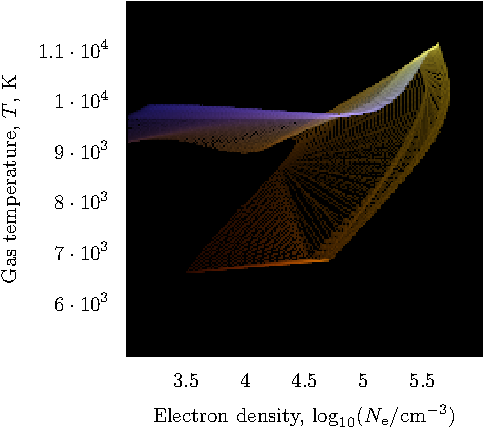
\includegraphics[width=0.45\linewidth]{NT-plane-SNO-RGB} &
    \includegraphics[width=0.465\linewidth]{Ne-Te-overlay}
  \end{tabular*}
  \caption[]{Emission structure in the \(n\elec\)--\(T\elec\) plane for the example physical model of 177-341.  
    (\textit{a})~Positive-colored image of the three emission lines: [\sii] \SI{6731}{\AA} (red), [\nii] \SI{6584}{\AA} (green), and [\oiii] \SI{5007}{\AA} (blue), with brightness proportional to the fraction of the model luminosity in each line that comes from gas with that particular combination of density and temperature.  
The variations in density and temperature within the model are principally a function of radius within the proplyd, with a secondary variation as a function of angle between the ``nose'' and the ``ears'' of the proplyd crescent due to the increasing obliqueness of the illumination angle.  
The outer zones of the model are at low density and are highly ionized, emitting principally in [\oiii], as seen in the blue horizontal branch at \(\simeq \SI{9700}{K}\) in the upper left part of the figure.  
As one approaches the proplyd ionization front (direction of increasing density), the [\nii] and then [\sii] emission become relatively stronger (color changes to yellow) and the temperature increases, reaching a maximum of \(\simeq \SI{11000}{K}\).  
In the ionization front itself, the temperature drops while the electron density climbs to a peak of about \SI{3e5}{cm^{-3}} and then also falls.  At the same time, the [\sii] emission comes to dominate over [\nii], giving rise to the orange-red branch that curves down and to the left.  
(\textit{b})~Negative-colored image of the same data as in \textit{a} overlayed with the observational diagnostic curves from Fig.~7\textit{a}.  The white star shows the solution for \(n\elec, T\elec\) obtained in \S~XX under the assumption that the emission in all three ions is co-extensive at a single density and temperature.  
}
  \label{fig:model:nT}
\end{figure*}

\begin{figure*}
  \centering
  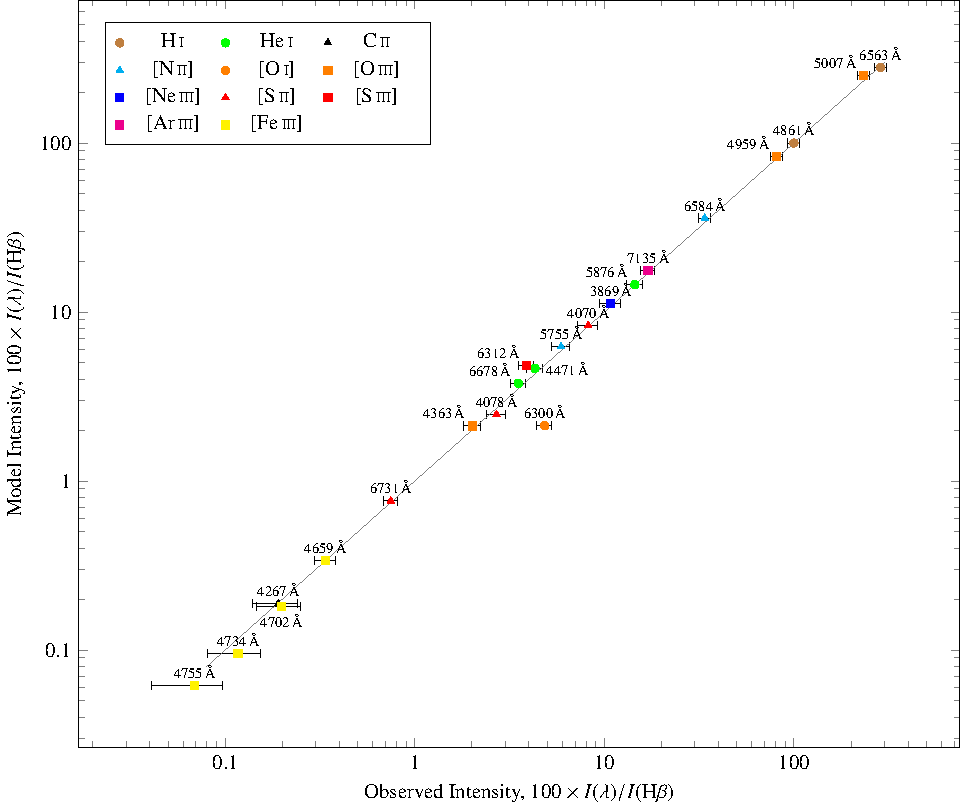
\includegraphics[width=\linewidth]{ratios-figure-figure10}
  \caption{Comparison of model and observed line intensities for 177-341.  
  }
  \label{fig:model}
\end{figure*}


Preliminary results of the emission line spectrum of such a model applied to 177-341 are shown in Figures~\ref{fig:model:nT} and \ref{fig:model}.  
The input parameters for the model (values given in Table~\ref{tab:model:pars}) are the radius of the ionization front at the proplyd cusp (assumed hemispherical), the intensity and spectral shape of the illuminating stellar radiation, and the composition (gas-phase elemental mix and dust grain populations) of the proplyd material.
For most of these parameters, we have taken values from the literature, whereas the gas-phase abundances and incident ionizing flux have been adjusted slightly in an attempt to reproduce the observed emission line intensities. 
The stellar spectrum is that determined for the ionizing star \thC{} by spectroscopic analysis \citep{2006AandA...448..351S}. 
The ionization front radius is the value determined by fitting to \textit{HST} emission line images \citep{1999AJ....118.2350H}, while the adopted ionizing flux at the proplyd position corresponds to a physical separation of the proplyd from the ionizing star of \SI{2.13e17}{cm} if there is no intervening absorption.
Given the observed angular separation of \(25.84''\) \citep{1998AJ....116..293B}, and assuming a distance to the Orion Nebula of 440~pc (\citealp{2008AJ....136.1566O}, Appendix~A), the projected separation is \SI{1.70e17}{cm}, implying an inclination angle of \(\simeq 55^\circ\). 
The diffuse radiation field and the proplyd tail are ignored in this model, since the observational aperture (\S~2.2) only covers the head of the proplyd. 

Figure~\ref{fig:model} shows that the model generally reproduces very well the observed relative line intensities for 177-341.  

{\bfseries\boldmath\color{red!50!black}
\subsection*{STILL TODO}
  \begin{itemize}
  \item Replace figures with model with lower O abundance
  \item Discuss failure to reproduce [\ion{O}{1}] -- possible dissociation component that is not include in model
  \item Discuss marginal problem with [\ion{S}{3}] -- details of stellar atmosphere spectrum, WMBasic vs Tlusty
  \item Discuss Figure~\ref{fig:model:nT} vs Figure~7a.  Fact that the intersection of the three curves in Figure~7 is not the correct solution (according to our model) since the three ions [\oiii], [\nii], and [\sii] come from different regions with different \(n\elec\), \(T\elec\). 
  \item Discuss fact that model is only representative and abundance values are not necessarily reliable (especially where only one ion stage is observed)
    \begin{itemize}
    \item should take into account aperture more carefully
    \item need to investigate effects of varying dust properties
    \item internal extinction within the proplyd flow
    \item need to constrain with additional existing observations (HST imaging; velocity profiles; mid-IR emission)
    \end{itemize}
  \end{itemize}
}




\bibliographystyle{mn2e}
\bibliography{BibdeskLibrary}

\end{document}
